%theoretical.tex
% Theoretical Background %

\section{Ab Initio Many Body Quantum Mechanics}
 The first task of quantum chemistry is to formulate mathematics that can describe molecular systems through the physics of non-relativistic electrons and nuclei. This is accomplished through Hamiltonian mechanics acting on a set of functions, a basis, dubbed the Schr{\"o}dinger equation(SE).
   \begin{equation}
    \hat{H}\ket{\Psi} = E\ket{\Psi}
   \end{equation}
  The time-independent SE the full Hamiltonian is formed in the lens of electrostatic interactions of electrons and nuclei.  This formulation brings about the first approximation in quantum mechanics, the Born-Oppenheimer approximation.\cite{SzaboAttila1982}  Because of the difference in mass between nuclei and electrons, there is a disparity in their relative motion.  Thus one can decide to gauge the full problem in the realm of either a fixed nuclear field with point charge electron coordinates or an average field of electronic charge with nuclei embedded within. To be consistent with the mathematic formulation of electronic structure theory this paper will only consider the problem of explicit electrons coordinate systems with fixed nuclear position.  The approximation allows one to neglect the kinetic energy of nuclei and consider nuclear-nuclear repulsion as a constant.  What is left is the N-body electronic Hamiltonian
   \begin{equation}
    \hat{H}_{elec} = -\sum_{i=1}^{N} \frac{1}{2} \nabla_{i}^{2} - \sum_{i=1}^{N}\sum_{A=1}^{M} \frac{Z_A}{r_{iA}} + \sum_{i=1}^{N}\sum_{j>i}^{N} \frac{1}{r_{ij}}
   \end{equation}
  The first term in this expression is the kinetic energy operator applied to N electrons, the second is the potential energy operator between electron-nuclei pairs and the final term is the potential energy operator of electron-electron pairs.  This Hamiltonian can be used to solve the electronic Scr{\"o}dinger equation
    \begin{equation}
     \hat{H}_{elec} \ket{\Psi_{elec}} = E_{elec}\ket{\Psi_{elec}}
    \end{equation}
  With the electronic wavefunction, $\Psi_{elec}$, dependent explicitly on the position of electrons and implicitly on the position of the nuclei.  Because $E_{elec}$ depends parametrically on the position of the nuclei, the total energy of the system can be calculated as 
    \begin{equation}
      E_{tot} = E_{elec} + \sum_{A=1}^{M} \sum_{B>A}^{M} \frac{Z_A Z_B}{R_{AB}}
    \end{equation}
  Though the full multi variable partial differential SE defined above is simplified with the Born-Oppenheimer approximation, it is still too complicated to solve for systems with more than one electron.\cite{SzaboAttila1982}
  \subsection{Hartree-Fock}
    Though it may not be possible to analytically solve the SE for an arbitrary number of electrons, it is able to exactly solve the differential for one electron.  The idea of solving the SE in a basis of N-tuple single electron functions is the fundamental basis for an approximate solution, known as Hartree-Fock (HF) theory. \cite{Hartree1928,Fock1930,SzaboAttila1982,Sherril2000} This approximation implies that one can express the electronic wavefunction, $\Psi_{elec}$, as an antisymmetric product of one electron functions, molecular orbitals (MO), that depend on the coordinate, $x = \{\vec{r}, \omega\}$, which contains spacial, $\vec{r}$, and spin, $\omega$, coordinates. Formally the antisymmetric wavefunction is constructed using a Slater determinant\cite{Slater1929,Slater1930} 
    \begin{equation}
    \Psi_{0}(x_1, x_2, ..., x_N) = \frac{1}{\sqrt{N!}}
    \begin{vmatrix}
     \chi_i(x_1) &\chi_j(x_1) &\ldots   &\chi_k(x_1)   \\
     \chi_i(x_2) &\chi_j(x_2)  &\ldots & \chi_k(x_2)   \\
     \vdots&\vdots   &\vdots &\vdots   \\
     \chi_i(x_N) &\chi_j(x_N) & \ldots & \chi_k(x_N)
    \end{vmatrix}
    \end{equation}
    This mathematical formalism introduces exchange correlation to electrons characterized by the same spin variable.  Though electrons of opposite spin are a simple uncorrelated product of one another.
    
    The best approximate solution can be found by variationally minimizing the Rayleigh quotient
      \begin{equation}
      E_{0} = \frac{\bra{\Psi_{0}} \hat{H}_{elec} \ket{\Psi_{0}}}{\selfolap{\Psi_{0}}}
      \end{equation}
    held to the constraint that
      \begin{equation}
        \olap{ \chi_i}{\chi_j} = 
          \begin{cases}
          1  & \quad i=j\\
          0  & \quad i\neq j
          \end{cases}
      \end{equation}
    and where the bracket notation implies the Hilbert space inner product.  The inner product $\bra{\Psi_{o}} \hat{H}_{elec} \ket{\Psi_{0}}$ is a set of eigenvalue integro-differential equation over all space, the HF equations, with each element defined as 
      \begin{equation} \label{Fock_eq}
      \hat{f}\chi_i = \epsilon_i \chi_i
      \end{equation}
    $\hat{f}$ the Fock operator is an effective one-electron operator of the form 
      \begin{equation} \label{Fock_op}
      \hat{f}(x_1) = \hat{h}_i(x_1)  + \sum_{j\neq i}^N \hat{J}_j(x_1) - \hat{K}_j(x_1)
      \end{equation}
    where $\hat{h}(x_1)$ is the average kinetic and nuclear attraction energy of a single electron and is expressed as 
      \begin{equation} \label{h}
      \hat{h}(x_1) = -\frac{1}{2} \nabla_1^2 - \sum_{A=1}^M \frac{Z_A}{r_{1A}}
      \end{equation}
    The last two terms in \cref{Fock_op} represent the potential energy of the electron-electrons interaction. $\hat{J}_j$ represents the Coulombic repulsion between two electrons
      \begin{equation} \label{j}
      \hat{J}_j(x_1) = \int \chi_j^*(x_2) \frac{1}{r_{ij}} \chi_j(x_2) dx_2
      \end{equation}
    $\hat{K}_j$, the exchange term, does not have a classical representation as the previous terms do and is direct product of the antisymmetric nature of the single determinant wavefunction
      \begin{equation} \label{k}
      \hat{K}_j(x_1) = \int \chi_j^*(x_2) \frac{1}{r_{ij}} \chi_i(x_2) dx_2
      \end{equation}
    The solution to the HF equation provides a set of orthonormal spin orbitals, $\{ \chi_k \}$, each with orbital energy $\{\epsilon_k\}$.  In principle there are infinitely many solutions to \cref{Fock_eq}, though in a finite basis there exists K spatial orbitals giving rise to 2K spin orbitals.  The solution to the HF eigenvalue problem provides N occupied and 2K-N unoccupied orbitals.
    %Larger basis sets variationally reduce the Hartree-Fock Energy, $E_0$, to the Hartree-Fock limit and will be useful in methods such as configuration interaction and coupled cluster.\cite{Szabo 1996}  \\
    
    %To numerically solve the HF eigenvalue equation one must define the one electron orbital functions $\{\chi_k\}$.  
    The solutions of the Hydrogen atom define one electron orbital functions, $\{\chi_k\}$, exactly as Slater type orbitals. Unfortunately, numerical differentiation, integration and finding distinct functional solutions to the HF equations using Slater type orbitals provides a formidable challenge. In order to produce a simplified solution one expands MO basis functions into M atomic orbital (AO) basis functions
      \begin{equation} \label{AO_eq}
      \chi_i = \sum_\mu^M C_{i\mu} \phi_\mu(x)
      \end{equation}
    where $\phi_\mu$ are typically atom centered functions.  Applying \cref{AO_eq} to \cref{Fock_eq} produces what is known as the Hartree-Fock-Roothaan matrix equation\cite{Roothaan 1960,Roothaan 1951}
      \begin{equation} \label{Rooth}
      \textbf{FC} = \textbf{SC}\epsilon
      \end{equation}
    \textbf{C} is the transformation matrix from \cref{AO_eq}, \textbf{S} is the overlap of two AO's
      \begin{equation}
      S_{\mu\nu} = \int \phi^*_\mu(x_1) \phi_\nu(x_1) dx_1
      \end{equation}
    and elements of the Fock matrix, \textbf{F}, are
      \begin{equation}
      F_{\mu\nu} = \int \phi_\mu(x_1) \hat{f}(x_1) \phi_\nu(x_1) 
      \end{equation}
    The Fock matrix terms can also be expanded with respect to the operators defined in \cref{h,j,k}:
      \begin{equation}
      F_{\mu\nu} = h_{\mu\nu} + \sum_{occ}\sum_{\rho \sigma} C_{\rho i} C_{\sigma i} \bra{\mu \rho}\ket{\nu \sigma}
      \end{equation}
    where 
      \begin{equation}
      \bra{\mu \rho}\ket{\nu \sigma} = \olap{\mu \rho}{\nu \sigma} - \olap{\mu \rho}{\sigma \nu}
      \end{equation}
    is the antisymmetrized difference of the coulomb and exchange terms with 
      \begin{equation} \label{antisymm}
      \olap{\mu \rho}{\nu \sigma} = (\mu \nu | \rho \sigma) = \int \int \phi^*_\mu(x_1) \phi^*_\rho(x_2) \frac{1}{r_{12}} \phi_\nu (x_1) \phi_\sigma(x_2) dx_1 dx_2
      \end{equation}
    in physicist and chemist notation, respectively. Roothaan's equation \cref{Rooth} specifies HF as a system of non-linear equations and must be solved iteratively to optimize expansion coefficients in a self-consistent-field (SCF) procedure. Computationally evaluation of the Fock matrix is the most expensive step of HF with asymptotic scaling of $\mathcal{O}(N^4)$ or $\mathcal{O}(N^2(lnN)^2)$ for large systems where N is the number of electrons and a storage requirement of $\mathcal{O}(N^4)$.  
  \subsection{Electronic Correlation Methods}
    Correlation is a concept of probability. Two variables are considered independent if the joint probability of the variables is a product of each variables probability; $p(x,y) = p(x) \times p(y)$ where $p(\cdot)$ is a probability function.  Otherwise, the two variables are said to be correlated.\cite{Kutzelnigg2003}  Electron correlation develops from %antisymmetric and indistinguishable%
    properties of fermions and Coulombic repulsion between electronic charges. HF does cannot recover electron correlation beyond the fermionic description.  The wavefunction in HF theory relies on the independent particle model, by definition this is an uncorrelated description as it does not consider electron-electron repulsion explicitly but as %electron repulsion with an average electron cloud charge.  
    field effect. Correlation energy, as defined by L{\"o}wdin \cite{Lowdin1959}, is 
      \begin{equation} \label{corr_E}
      E_{corr} = \mathcal{E}_{0} - E_{HF}
      \end{equation}
    Where $\mathcal{E}_0$ is the exact non-relativistic energy and $E_{HF}$ is energy recovered at the HF limit.  This definition is imprecise; it may be more useful to think of $E_{corr}$ as an observable of some quantum mechanical operator acting on wavefunction with the form:
      \begin{equation}
      \Psi_{exact} = \Psi_{HF} + \Psi_{corr}
      \end{equation}
    where $\Psi_{corr}$ is orthogonal to $\Psi_{HF}$ and encapsulates all correlation not captured by HF.\cite{Kong2012}  Though correlation energy only contributes a very small portion to the total energy, these corrections are extremely necessary in the accurate calculation of molecular properties and prediction of reactions.  Outlined to follow are a methods that allow theoretical chemistry to systematically calculate correlation energy.
    \subsubsection{Many Body Perturbation Theory}
      Many Body Perturbation Theory (MBPT) was first developed in 1957\cite{Brueckner1955} to study the energy of nuclear matter.  Not until 1968 was the it applied to ab initio quantum chemistry.\cite{Freed1968,Freed1971}.  Though there are many formulations of MBPT, two of the most well known being Rayleigh-Schr{\"o}dinger\cite{Lindgren1974} and M{\/o}ller-Plesset\cite{Moller1934, Raghavachari1989}, all methods are developed from the same principles.  %The distinction comes from the use of diagrams and the definition of the zeroth order hamiltonian and perturbative potential.  
      The formulation presented will follow the M{\/o}ller-Plesset (MPn) definition of MBPT, where n is the perturbative order correction. 
      MBPT is not variational, the solution recovered from an approximation is lower bounded by the exact energy, but is size consistent.       %check the validity of this statement}
      For a method to be size consistent it must be able to calculate the energy of two elements, separated by infinite distant to be the sum of its individual parts.  
        \begin{equation}
        	E_{r=\infty}(AB) = E(A) + E(B)
        \end{equation}
      Starting with an eigenvalue problem
        \begin{equation} \label{eigenvalue}
        	\hat{H}\ket{\Phi} =  E\ket{\Phi}
        \end{equation}
      one can expand the eigenvalue operator
      \begin{equation}
      	\hat{H} = \hat{H}^{(0)} + \lambda \hat{H}^{(1)}
      \end{equation}
      $\hat{H}^{(0)}$, the zeroth order operator, is assumed to closely approximate the exact Hamiltonian and $\hat{H}^{(1)}$ is the perturbative, first order correction to the zeroth order problem. One can then expand the wavefunction and energy
        \begin{equation}
        	\ket{\Phi} = \ket{\Phi^{(0)}} + \lambda \ket{\Phi^{(1)}} +  \lambda^2 \ket{\Phi^{(2)}} + \dots\\
        \end{equation}
        \begin{equation}
        	E = E^{(0)} + \lambda E^{(1)} + \lambda^2 E^{(2)} + \dots
        \end{equation}
       Applying these expansions to \cref{eigenvalue} and accumulating terms of a single order, $\lambda^n$, one finds
         \begin{equation}\label{mpn}
         	  \hat{H}^{(0)}\ket{\Phi^{(n)}} + \hat{H}^{(1)}\ket{\Phi^{(n-1)}} = \sum_{i=0}^n E^{(i)} \ket{\Phi^{(n-i)}}
        \end{equation}  
      MPn theory assumes %HF is the zeroth order solution to the SE eigenvalue problem.%solution close to the exact energy of a system.
        \begin{equation}\label{h0}
          \hat{H}^{(0)} = \sum_{i=1}^N \hat{f}(i) = \sum_{i=1}^N \hat{h}(i) + \hat{J}(i) - \hat{K}(i)
        \end{equation}
      and defines the first order correction as 
        \begin{equation}\label{h1}
          \hat{H}^{(1)} = \hat{H}_{elec} - \hat{H}^{(0)} = \sum_{i<j} \frac{1}{r_{ij}} - \sum_i (\hat{J}(i) - \hat{K}(i))
        \end{equation}
     % Through left project one can find energy equations
        %\begin{equation}\label{proj}
          %\begin{aligned}
           % \bra{\Phi^{(0)}}\hat{H}^{(0)}\ket{\Phi^{(0)}} &= E^{(0)}\\
            %\bra{\Phi^{(0)}}\hat{H}^{(1)}\ket{\Phi^{(0)}} &= E^{(1)}\\
            %\bra{\Phi^{(0)}}\hat{H}^{(1)}\ket{\Phi^{(1)}} &= E^{(2)}\\
            %&\vdots
          %\end{aligned}
        %\end{equation}
      MPn theory typically focuses on solving second order correction, MP2; first order corrections are zero by Brillouin theorem \cite{surjan1989}.  Substituting \cref{h0,h1} into \cref{mpn} one finds 
        \begin{equation}
          \bra{\Phi^{(0)}}\hat{H}^{(0)}\ket{\Phi^{(0)}} = \sum_{i=1}^N \epsilon_i = E^{(0)}
        \end{equation}
        where $\Phi^{0} = \Psi_0$ the lowest energy HF reference state 
        \begin{equation}
           \bra{\Phi^{(0)}}\hat{H}^{(1)}\ket{\Phi^{(1)}} =\bra{\Phi^{(0)}}(\hat{H}_{elec} - \hat{H}^{(0)}) \ket{\Phi^{(1)}}  =  E^{(2)}
         \end{equation}
       Where $\epsilon_i$ are the HF orbital energy coefficients. $\Phi^{(1)}$ is expanded in terms of eigenvectors of $\hat{H}^{(0)}$.  Slater-Condon rules\cite{SzaboAttila1982} determine %say that, because all the terms in $\hat{H}^{(1)}$ are two particle operators, the right wavefunction and left projection can only differ by two terms.  Thus 
       %the only non-zero basis orthogonal to $\Psi_0$ is the 
       $\ket{\Phi^{(1)}}$ must be from the set of double excited reference state determinant, $\ket{\Psi^{ij}_{ab}}$. Where terms of the form $\ket{\Psi^{ijk\dots}_{abc\dots}}$ are created by replacing HF MO $\chi_i$ in the set N occupied orbital with an orbital $\chi_a$ from the next set of 2K-N unoccupied orbitals and so on.  This provides the expansion 
         \begin{equation} \label{phi1}
          \ket{\Phi^{(1)}} 
          %= \sum_{\substack{i<j\\a<b}} \ket{\Psi^{ij}_{ab}} \olap{\Psi^{ij}_{ab}}{\Phi_0}  
          %= \frac{1}{4} \sum_{ijab} \ket{\Psi^{ij}_{ab}} \olap{\Psi^{ij}_{ab}}{\Phi_0} 
          = \frac{1}{4}\sum_{ijab} t^{ij}_{ab} \ket{\Psi^{ij}_{ab}}
        \end{equation}
      projecting \cref{phi1} onto the first order energy equation, one can find the coefficient $t^{ij}_{ab}$ then solve the second order energy equation %in the canonical molecular orbital basis to find
        \begin{equation}
          E^{(2)} = \frac{1}{4} \sum_{ijab} \frac{\bra{ij}\ket{ab}}{\epsilon{(i) + \epsilon(j) - \epsilon(a) - \epsilon(b)}}
        \end{equation}
      The term $\bra{ij}\ket{ab}$ from \cref{antisymm} has been transformed by
        \begin{equation}
          \bra{ij}\ket{ab} = \sum_{\mu\nu\rho\sigma} C_{\mu i} C_{\nu j} C_{\rho a} C_{\sigma b} \bra{\mu \nu} \ket{\rho \sigma}
        \end{equation}
      This transformation is the most computationally rigorous step of MP2 scaling as $\mathcal{O}(N^5)$ with a storage requirement of $\mathcal{O}(N^4)$.  Efforts to eliminate the transformation using the Laplace transformation (LT) will be discussed in detail in the research section.  Currently, LT-MP2's efficient reduction in computational cost has only been observed with sufficiently large molecules, more than 200 atoms.   
    %%%%%%%%%%%%%%%%%%%%%%%%%%%%%%%%%
    \subsubsection{Configuration Interaction}
      Configuration Interaction (CI) method is an application of the Ritz method of linear variations to the electronic wavefunction\cite{Shavitt1977,Ritz1909,Szabo1998}. CI methods diagonalize the N-electron hamiltonian in terms of $\Psi_{exact}$.  This can be achieved by expanding $\Psi_{corr}$ as a linear combination of all possible N-tuply excited slater determinants%slater determinants constructed from N electrons and 2K spin orbitals, $\{\chi_k\}$ 
        \begin{equation}\label{CI_wfn}
      	  \ket{\Psi_{exact}} = C_0\ket{\Psi_0} + \sum_{ia} C^i_a \ket{\Psi^i_a} + \sum_{\substack{i<j\\  a<b}} C^{ij}_{ab} \ket{\Psi^{ij}_{ab}} + \sum_{\substack{i<j<k \\ a<b<c}} C_{abc}^{ijk} \ket{\Psi_{abc}^{ijk}} + \dots 
        \end{equation}
      %Where  $\Psi_0$ represents the Hartree-Fock Slater determinant expressed in a some basis. 
      In an infinite basis this expansion provides an equality to $\Psi_{exact}$.  Though, in a finite basis there exists $\binom{N}{2K}$\cite{Szabo 1998} terms and the expansion is approximate. The coefficients C express the weighting of each slater determinants in the exact wavefunction expansion.  The exact wavefunction is not normalized though it does have intermediate normalization\cite{Szabo 1998} defined as 
        \begin{equation}
        \olap{\Psi_0}{\Psi_{exact}} = 1
        \end{equation}
      %One can apply SE to the exact wavefunction and find 
        %\begin{equation}
       	 %\hat{H}_{elec}\ket{\Psi_{exact}} = \mathcal{E}_0 \ket{\Psi_{exact}}
        %\end{equation}
      %Substituting in the definition from equation (19) to solve for $E_{corr}$ we find 
      Applying SE and substituting \cref{corr_E}, one finds
        \begin{equation} \label{CI_E}
        	(\hat{H}_{elec} - E_{HF})\ket{\Psi_{exact}} = (\mathcal{E}_0 - E_{HF})\ket{\Psi_{exact}} = E_{corr} \ket{\Psi_{exact}}
        \end{equation}
      Using intermediate normalization one can project \cref{CI_E} by the HF reference wavefunction and find 
        \begin{equation}
      	  \bra{\Psi_0}(\hat{H}_{elec} - E_{HF})\ket{\Psi_{exact}} = E_{corr}\olap{\Psi_0}{\Psi_{exact}} = E_{corr}
        \end{equation}
      then substituting \cref{CI_wfn} one finds
        \begin{equation}
        \bra{\Psi_0}(\hat{H}_{elec} - E_{HF})\ket{\Psi_{exact}} = \bra{\Psi_0}(\hat{H}_{elec} - E_{HF})\ket{\Psi_0} + \sum_{\substack{i<j \\ a<b}}C^{ij}_{ab}\bra{\Psi_0}\hat{H}_{elec}\ket{\Psi^{ij}_{ab}} + \dots
        \end{equation}
      by Slater-Condon rules one finds
        \begin{equation}
        \sum_{\substack{i<j \\ a<b}}C^{ij}_{ab}\bra{\Psi_0}(\hat{H}_{elec})\ket{\Psi^{ij}_{ab}}  = E_{corr}
        \end{equation}
      To resolve $C^{ij}_{ab}$ it is necessary to project excited determinants onto \cref{CI_E}
        \begin{equation}\label{long_eq}
        	\begin{aligned}
        		\bra{\Psi^{ij}_{ab}}(\hat{H}_{elec} &- E_{HF})\ket{\Psi_{exact}} = \bra{\Psi^{ij}_{ab}}(\hat{H}_{elec} )\ket{\Psi_0} +  \sum_{\substack{k\\c}} C^k_c\bra{\Psi^{ij}_{ab}}(\hat{H}_{elec} )\ket{\Psi^k_c} \\
      		&+  \sum_{\substack{k<l \\ c<d}}C^{kl}_{cd}\bra{\Psi^{kl}_{cd}}(\hat{H}_{elec}-E_{HF})\ket{\Psi^{ij}_{ab}}  +\dots\\
          %+  \sum_{\substack{k<l<m \\ c<d<e}}C^{klm}_{cde}\bra{\Psi^{klm}_{cde}}\hat{H}_{elec}\ket{\Psi^{ij}_{ab}} \\
      	%	&+  \sum_{\substack{k<l<m<n \\ c<d<e<f}}C^{klmn}_{cdef}\bra{\Psi^{klmn}_{cdef}}\hat{H}_{elec}\ket{\Psi^{ij}_{ab}} \\
          	&= C^{ij}_{ab}E_{corr}
        	\end{aligned}
        \end{equation}
      \cref{long_eq} exemplifies how solving the CI energy equation requires one to iteratively solve $\binom{N}{2K}$ coupled equations.  
      %Thus, full-CI calculations are typically restricted to small molecules. 
      One can reduce the full-CI correlation energy calculation by truncating the set of CI coefficients, for example CI singles and doubles (CISD).  
      %This is done in configuration interaction singles and doubles (CISD), where one assumes that only $C^i_a$ and $C^{ij}_{ab}$ are non-zero.
      The CISD formulation has computational scaling of $\mathcal{O}(N^6)$ and storage requirement of $\mathcal{O}(N^4)$.  Any truncation to the full-CI method eliminates the size-consistency of CI methods.  Additionally, truncated CI is not size-extensive, meaning the energy calculated by truncated CI methods do not scale linearly with number of electrons, N; CI is variational.
      %Though the best ground state can be formed with a single determinant of the first N electron spin orbitals orbitals, $\{\chi_k\}$, the number of combination of orbitals is much larger. The other determinants can be taken 

      %The exact orbitals solved analytically from the electronic wavefunction expression of hydrogen are defined using slater orbitals.  In theoretical chemistry Slater type orbitals are approximate by linear combinations of Gaussian type orbitals.  
    %%%%%%%%%%%%%%%%%%%%%%%%%%%%%%%%%%%
    \subsubsection{Coupled Cluster Thoery}
      Since its development in the 1960's by {\u C}{\'i}{\u v}ek and Paldus \cite{Civek 1966, Civek 1969, Civek 1971} Coupled Cluster (CC) theory has become the most reliable method used for accurate approximations of atomic and molecular properties.\cite{Crawford 2000}.  The foundation of CC theory is based on exponential expression of the wavefunction
        \begin{equation}
          \ket{\Psi_{exact}} = e^{\hat{T}}\ket{\Phi}
        \end{equation}
      A power series expansion of the expression provides the following equation
        \begin{equation}
          e^{\hat{T}}\ket{\Phi} = (1 + \hat{T} + \frac{1}{2!} \hat{T}^2 + \frac{1}{3!} \hat{T}^3 + ...) \ket{\Phi}
        \end{equation}
      Where $\hat{T}$ is the cluster operator of the form 
        \begin{equation}
          \hat{T} = \hat{T}_1 + \hat{T}_2 + \hat{T}_3 + ... + \hat{T}_N
        \end{equation}
      the nth order cluster operator has the form 
        \begin{equation}
          \hat{T}_n = \left(\frac{1}{n!}\right)^2 \sum_{ij\dots,ab\dots}^{n} t_{ij\dots}^{ab\dots} a^\dagger_a a^\dagger_b \dots a_j a_i 
        \end{equation}
      where $a_i$ and $a^\dagger_a$ are the second-quantization operators. $a_i$ deletes an orbital $\phi_i$ and $a^\dagger_a$ inserts an orbital $\phi_a$ from the determinant which the operators act upon, $\chi_l$ %Therefore the cluster operators replace n orbitals, $\phi_i$, $\phi_j, \dots$ with $\phi_a$, $\phi_b,\dots$ respectively.
      \cite{Crawford 2000, Bartlett 2007}.
      By including all cluster operators in the expression of $\hat{T}$ one can form the exact wavefunction, though the number of terms and the computational scaling factor becomes quickly unmanageable.  To deal with this problem the cluster operator, $\hat{T}$ is truncated.  The derivation to follow will restrict the problem to the single and double cluster operators (CCSD)
        \begin{equation}
          \hat{T} = \hat{T}_1 + \hat{T}_2
        \end{equation}
      Therefore one defines
        \begin{equation}\label{CC_wfn}
          \ket{\Psi_{CC}} = e^{\hat{T}}\ket{\Psi_0}
        \end{equation}
      %Applying \cref{CC_wfn} to the SE one finds
        %\begin{equation}
         % \hat{H}\ket{\Psi_{CC}} = \hat{H} e^{\hat{T}} \ket{\Psi_0} = (E_0 + E_{corr}) e^{\hat{T}} \ket{\Psi_0} = E_{CC} \ket{\Psi_{CC}}
        %\end{equation}
      %Here the wavefunction, 
      %$\Phi$, is assumed to be the HF reference wavefunction, $\Psi_0$ and 
      with intermediate normalization, $\olap{\Psi_0}{\Psi_{CC}} = 1$. 
      %To obtain a more computationally friendly expression the the expression is left projected by $e^{-\hat{T}}$, providing a similarity transformed Hamiltonian.  
      Left projecting the SE by $e^{-\hat{T}}$ allows one to simplify the energy expression using the Cambell-Baker-Hausdorff formula\cite{crawford2000} and find%then provide computationally useful equations using the following equations 
        \begin{equation}\label{E_cc}
            E_{CC} = \bra{\Psi_0}e^{-\hat{T}} \hat{H} e^{\hat{T}} \ket{\Psi_0}
        \end{equation}
        \begin{equation}\label{t1}
          0 = \bra{\Psi^a_i} e^{-\hat{T}} \hat{H} e^{\hat{T}} \ket{\Psi_0}
        \end{equation}
        \begin{equation}\label{t2}
          0 = \bra{\Psi^{ab}_{ij}} e^{-\hat{T}} \hat{H} e^{\hat{T}} \ket{\Psi_0}
        \end{equation}
      where 
        \begin{equation}
          E_{CC} = E_0 + E_{corr}
        \end{equation}
      \cref{t1,t2} provide a set on nonlinear equations which must be solved iteratively to provide the single and double cluster amplitudes, $t^a_i$ and $t^{ab}_{ij}$.
      Coupled Cluster theory is not variational but is size-consistent and size-extensive.  
      CCSD scales as $\mathcal{O}(N^6)$ and inclusion of the triple cluster operator (CCSDT) increases scaling to $\mathcal{O}(N^8)$\cite{Noga 1987, Scuseria 1988} with storage requirements of $\mathcal{O}(N^4) \text {and} \mathcal{O}(N^6)$, respectively. Chemists have developed a way around this problem by applying perturbation theory to CC to include the triples operator\cite{Crawford2000}. 
      This approach scales as $\mathcal{O}(N^7)$ and is considered quantum chemistries gold standard.
  \subsection{Explicitly Correlated Methods}
    %It can be concluded that even when using the "gold standard" in quantum chemistry, CCSD(T), there still exists some error in our approximations.  
    Within quantum chemistries most accurate approximations one finds the largest contribution to error is the basis set error.  %The first place this error comes from is in the expression of one electron wavefunctions.  
    In the wavefunction framework established above, to achieve high accuracy in calculations one must enlist large basis sets and large $\zeta$.  Even so basis set error contributions have very slow convergence and fails to recreate the electron cusp condition.  Figure 1 shows the electron probability on a cross section of a sphere.  Because HF provides an average electronic field, the electrons probability is constant no matter the position of electron two.  While in truth there is zero probability of electron one at the point of electron two and higher probaility that electron one will be found $\pi$ radians away from electron two.  These corrections are known as Coulombic correlation. 
    \begin{figure}[H]
      \centering
        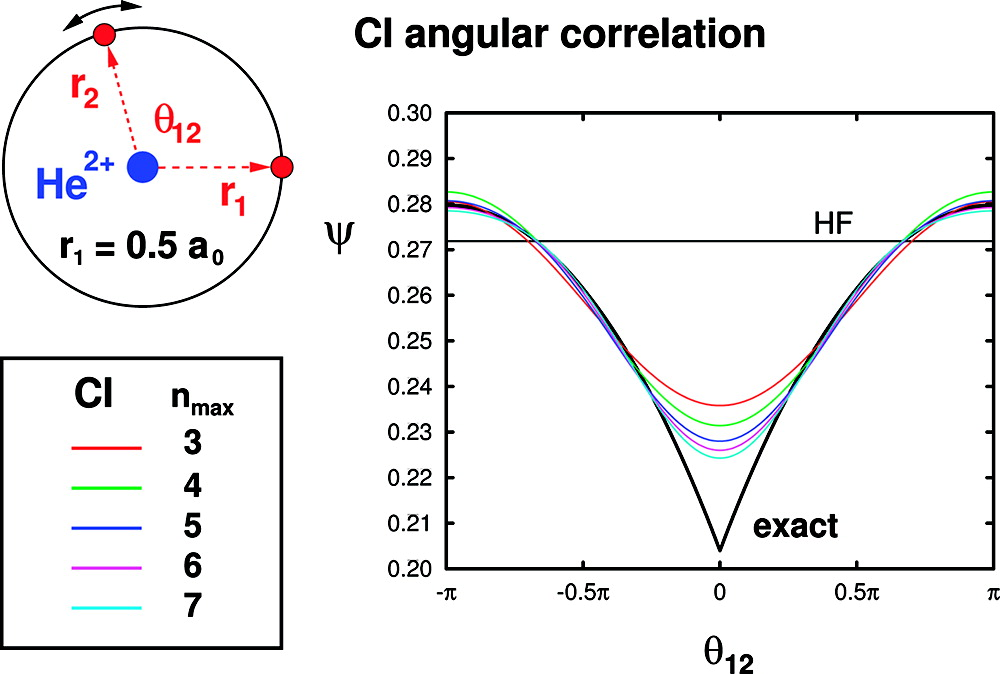
\includegraphics[width = 9cm, height = 6cm]{./pics/ang.jpeg}
        \caption{Electron-electron cusp condition for a Heliums ground state wavefunction with both electrons on the same circle of $.5 a_0$ using a CI based wavefunction with increasing basis size with maximum principle quantum number, $n_{max}$\cite{Hatting 2012}.}
    \end{figure}
    In order to more accurately calculate Coulombic correlation energy it is necessary to generate a new wavefunction expression that is explicitly dependent on inter-electronic distances. Kato's cusp condition\cite{kato 1957} comes from realizing the characterization of a first-order derivative discontinuity at the Coulombic type singularity\cite{Hatting 2012}. This fact provides the coalescence condition 
      \begin{equation}
          \left. \frac{\partial \Psi}{\partial r_{12}} \right |_{r_{12}=0} = - \frac{1}{2} \Psi(r_{12}=0)
        \end{equation}
    One assumes the form of the exact wavefunction is as follows:
      \begin{equation}
        \Psi_{exact}(r_1, r_2 , \dots) = \Phi(r_{12})\Psi(R_{12})
      \end{equation}
    Where $R_{12} \equiv \frac{r_1 + r_2}{2}$ and $r_{12} \equiv r_1 - r_2$ and the form of $\Phi{r_{12}}$ is chosen such that it satisfies the coalescence condition and 
      \begin{equation}
        \Phi(r_{12}) = R(r_{12})\Theta(\Omega_{12})
      \end{equation}
    The exact representation of the two electron portion, $\Phi(r_{12})$, can be solved through seperation of variables.  The angular portion, $\Theta(\Omega_{12})$, can be represented with the spherical harmonics, $Y_{lm}$, and the radial portion, $R(r_{12})$ can be solved using approximate solutions to the two-electron radial SE
      \begin{equation}
        \left( -\frac{1}{2r^2_{12}} \frac{\partial}{\partial r_{12}} r^2_{12} \frac{\partial}{\partial r_{12}} + \frac{l(l+1)}{2r^2_{12}} + \frac{1}{r_{12}} + \mathcal{O}(r^0_{12}) \right) R(r_{12}) = 0
      \end{equation}
    Solving this differential with appropriate ans{\"a}tz provides the approximate solution
      \begin{equation}
        \Psi(r_1, r_2, \dots) \approx r^l_{12} \sum_{m=-l}^l\left( 1 + \frac{r_{12}}{2(l+1)} + \mathcal{O}(r^2_{12})\right) Y_{lm}(\Omega_{12})\Phi(R_{12},\dots)
      \end{equation}
    In the first attempts to create a wavefunction that was explicitly dependent on inter-electronic distances by Hartree \cite{Hartree 1928} and Hylleras\cite{Hylleras 1929}, the cusp condition was unknown and therefore the attempts could not effectively create functions that could be efficiently calculated.  Incorporation of cusp condition has allowed the introduction of functions many types of functions such as Hylleraas-CI, explicitly correlated Gaussian, and many body Gaussian geminal type.\cite{Kong 2012}  The development of these methods has allowed F12/R12 to develop as a computational tool.
    In the next sections I will discuss the use of F12/R12 in MP2 and CC methods.
    %Hartree and Ingman, the form used in modern F12/R12 methods.\\ %\cite{Hartree, D. R.; Ingman, A. L. Mem. Proc. Manchester Lit. Philos. Soc. 1933, 77, 69}
    \subsubsection{Explicitly Correlated MP2 R12 method}
      The formal difference between MP2 and MP2 R12 methods are the definition of first order wavefunction.  In standard MP2 theory the first order wavefunction is expressed as equation (32).  MP2-R12's first order wavefunction includes this term and explicitly correlated geminal functions.
        \begin{equation}
          \ket{\Psi_{MP2-R12}} = \ket{\Phi^(1)_{MP}} + \sum_{\substack{i<j \\ x<y}} t^{ij}_{xy} \ket{\Psi^{ij}_{xy}}
        \end{equation}
      Where the geminal basis function are quasi-double excitations with respect to the reference, $\ket{\Psi_0}$
        \begin{equation}
        \ket{\Psi^{ij}_{xy}} = \frac{1}{2} \bar{R}^{\alpha \beta}_{xy} \tilde{a}^{\alpha \beta}_{i j} \ket{\Psi_0}
        \end{equation}
      Where $\tilde{a}^{\alpha\beta}_{ij}$ is the normal ordered, with respect to the reference state, string of creation and annihilation operators that produce a doubly excited state $\ket{\Psi^{ij}_{\alpha\beta}}$ and $\bar{R}^{\alpha\beta}_{xy}$ are matrix elements of the explicitly correlated factor, $f(r_{12})$ projected by a function, $\hat{Q}_{12}$, which ensure orthogonality of the excited geminal functions:
        \begin{equation}
          R^{\alpha \beta}_{xy} = \bra{\alpha \beta} \hat{Q}_{12} f(r_{12})\ket{xy}
        \end{equation}
      The most common choice for $\hat{Q}_{12}$, proposed by Valeev\cite{Valeev 2004} 
        \begin{equation}
          \hat{Q}_{12} = (1-\hat{O}_1)(1-\hat{O}_2)- \hat{V}_1 \hat{V}_2
        \end{equation}
      Other choices have also been considered \cite{wind 2002, Koppler 2002}.\\
      The doubly excited coefficients for the first order wavefunction can be solved for by minimizing Hylleraas functional for the second order MP energy 
        \begin{equation}
          H^{(2)} (\Phi^{(1)}) = \bra{\Phi^{(1)}} \hat{H}_0 - E_0 \ket{\Phi^{(1)}} + 2 \bra{\Phi}\hat{H}\ket{\Phi^{(0)}}
        \end{equation}
      using a modified one-step inversion of the zeroth Hamiltonian.  After solving for these coefficients $E_{\text{MP2-R21}}$ is 
        \begin{equation}
          E_{\text{MP2-R12}} = \bra{\Phi^{(0)}} \hat{H}^{(1)} \ket{\Phi^{1}} = E^{(2)}_{MP2} + E^{(2)}_{R12}
        \end{equation}
      The integrals of $E^{(2)}_{R12}$ can be solved analytically if the correlation factor, $f(r_{12})$, is Gaussian\cite{Polly 2006}.  The terms in $E^{(2)}_{R12}$ do require approximations to calculated fast and accurately some of which will be discussed later\cite{Kong 2012}.
    \subsubsection{Explicitly Correlated CC R12 method}
      It is necessary to apply R12 methods to CC in order to achieve the theories full potential because MP2-R12 has limited chemical framework\cite{kong 2012}.  CC-R12 extends the standard CC cluster operator, $\hat{T}$, to include R12 geminal operator, $f(r_{12})$\cite{Noga 1992, Noga 1994}.  For example the CCSD-R12 wavefunction has the form 
        \begin{equation}
          \ket{\Psi_{exact}} = e^{\hat{T}}\ket{\Psi_0}
        \end{equation}
      Where $\hat{T}$ has the form
        \begin{equation}
          \hat{T} = \hat{T}_1 + \hat{T}_2 + \hat{R}
        \end{equation}
      The operators $\hat{T}_1 \text{ and } \hat{T}_2$ are defined using equation (45) and $\hat{R}$ is defined as 
        \begin{equation}
          \hat{R} = \frac{1}{(2!)^3} t^{xy}_{ij} \bar{R}^{\alpha \beta}_{xy} \tilde{a}^{ij}_{\alpha \beta}
        \end{equation}
      where $\bar{R}^{\alpha \beta}_{xy}$ is the conjugate matrix element of the explicitly correlated factor defined in equation (59).
      The energy and amplitudes of the CC equation are found in the same fashion described in section 2.2.3 with the added projection of excited geminal functions using the operator $\tilde{\gamma}^{xy}_{ij}$
        \begin{equation}
          \ket{\Psi^{xy}_{ij}} \equiv \tilde{\gamma}^{xy}_{ij}\ket{\Psi_0} = \frac{1}{2!} \bar{R}^{\alpha \beta}_{xy} \tilde{a}^{ij}_{\alpha \beta}
        \end{equation}
      This creates an additional projection term
        \begin{equation}
          \bra{\Psi^{xy}_{ij}} e^{\hat{T}} \hat{H} e^{\hat{T}} \ket{\Psi_0} = 0
        \end{equation}
      Though this additional amplitude equation does have small store dimension, $\mathcal{O}(o^4)$ the computational complexity to implement CCSD-R12 is much greater than CCSD and MP2-R12, with CCSD-R12 scaling as $\mathcal{O}(N^8)$ with storage requirement of $\mathcal{O}(N^6)$.  Scaling can be reduced to $\mathcal{O}(N^6)$ with direct computation of an intermediate each iteration.\cite{Kong 2012} 